\documentclass[10pt, a4paper, twocolumn]{article}
\usepackage[utf8]{inputenc}
\usepackage{graphicx}
\usepackage{geometry}
\usepackage{times}
\usepackage{cite}
\usepackage{amsmath}
\usepackage{amssymb}
\usepackage{booktabs}
\usepackage{multirow}
\usepackage{url}
\usepackage{hyperref}
\usepackage{enumitem}
\usepackage{tikz}
\usetikzlibrary{positioning, fit, backgrounds}
\usepackage{xcolor}
\usepackage{algorithm}
\usepackage{algpseudocode}
\usepackage{caption}
\usepackage{subcaption}

\DeclareUnicodeCharacter{0001}{}

\geometry{top=2cm, bottom=2cm, left=1.5cm, right=1.5cm}
\setlength{\emergencystretch}{3em}
\sloppy
\hfuzz=30pt
\hbadness=10000

\hypersetup{
    colorlinks=true,
    linkcolor=blue,
    citecolor=blue,
    urlcolor=blue
}

\title{\textbf{MANJU: A Multi-Agent Framework for Natural Just-in-Time Understanding in Thai Voice-Based Customer Service}}

\author{
    Sawit Koseeyaumporn, Siratee Saiprom, Sansiri Tarnpradab \\
    \textit{Department of Computer Engineering} \\
    \textit{King Mongkut's University of Technology Thonburi} \\
    \textit{Bangkok, Thailand} \\
    \texttt{\{sawit.kosee, siratee.saip, sansiri.tar\}@kmutt.ac.th}
}

\date{}

\begin{document}

\maketitle

\begin{abstract}
This paper presents \textbf{MANJU} (Multi-Agent AI for Natural
Just-in-Time Understanding), an automated platform that handles
Thai-language customer service through real-time voice interaction.
Customer service operations often struggle with staff shortages and
long wait times during busy periods; MANJU addresses this by letting
an AI system listen to a customer's spoken question, reason about the
best answer, search relevant documents for supporting facts, and reply
in a natural Thai voice --- all within five seconds.

Users can customise the system's behaviour through a drag-and-drop
workflow editor that requires no programming. Behind the editor, the
platform chains together specialised AI components: speech recognition
converts voice to text, a group of cooperating AI agents decides how
to handle the query, a document search grounds the answer in real
sources to reduce errors, and a voice synthesis model reads the
response aloud with a cloned or preset voice.

In tests on a set of 50 Thai customer-service queries, MANJU correctly
routed 94\% of questions to the right handler, and the retrieved-context
approach raised factual accuracy from 50\% to 88\% compared with
using the language model alone. The voice output was generated faster
than real time, and the full end-to-end response consistently arrived
within the five-second target.
\end{abstract}

\vspace{0.5em}
\noindent\textbf{Keywords:} Multi-Agent System, Voice AI, Thai NLP,
Retrieval-Augmented Generation, Text-to-Speech, Customer Service
Automation, LangGraph.

% ===========================================================================
\section{Introduction}
% ===========================================================================

Most people today expect to get help from a business at any hour, not
just during office hours.
Yet phone-based customer service has not kept up: when call volumes spike,
there are simply not enough staff to respond quickly, which leaves
customers waiting and businesses losing opportunities~\cite{gans2003callcenters}.

AI can fill this gap by handling routine questions automatically, freeing
human agents for cases that genuinely need human judgment.
The problem is that most AI customer-service tools today are either
text-only chatbots or old-style phone menus (IVR systems) that follow
a fixed script.
Neither can hold a natural voice conversation, look up information from
a live document, or speak in a personalised voice~\cite{manjuProgReport}.

This paper introduces \textbf{MANJU}, a voice assistant built specifically
for Thai-language customer service.
A customer speaks a question; MANJU transcribes it, reasons about the
best answer, searches relevant documents for supporting facts if needed,
and replies in a natural Thai voice --- all within five seconds.
What sets MANJU apart is that the entire conversation logic is configured
visually: a non-technical operator drags and drops nodes in a browser
editor to define how queries are handled, and the system compiles that
design into a running AI workflow automatically, with no code changes
required.

\subsection{Objectives}

This work has four goals.
\begin{enumerate}[label=(\roman*)]
    \item Build a complete pipeline --- from listening to the customer's
          voice all the way to speaking a reply --- that responds in under
          five seconds.
    \item Provide a drag-and-drop editor so that non-developers can
          configure the AI workflow, choose knowledge sources, and select
          output formats without writing code.
    \item Ground every answer in real documents or live spreadsheet data
          to reduce the chance of the AI inventing incorrect information.
    \item Test the system on Thai customer-service questions and measure
          how fast it responds, how often it routes queries correctly, and
          how factually accurate its answers are.
\end{enumerate}

\subsection{Scope}
The current scope covers an MVP supporting FAQ, product information, and knowledge-base inquiries in Thai.
Four workflow modalities are supported: text-to-text, text-to-voice, voice-to-text, and voice-to-voice.
The scope excludes complex multi-turn stateful conversations, emotion analysis, CRM/ticketing integration, and domain-specific model fine-tuning.
The system operates on mixed CPU/GPU resources and supports browser-based voice access~\cite{manjuProgReport}.

\subsection{Contributions}
The contributions of this work are four-fold:
\begin{enumerate}[label=(\roman*)]
    \item \textbf{Workflow-as-Data Architecture:} A visual graph editor that compiles drag-and-drop node configurations into LangGraph \texttt{StateGraph} instances with eight node types and conditional branching.
    \item \textbf{Multi-Agent Orchestration:} LangGraph-based execution supporting intent routing, RAG enrichment, Google Sheets integration, and conditional logic within a single unified state machine.
    \item \textbf{Thai Voice Pipeline:} Integration of Web Speech API with custom VAD for input, and Qwen3-TTS-12Hz-1.7B with sentence-level streaming and voice cloning for output.
    \item \textbf{Production-Grade Platform:} A four-tier microservice deployment with JWT/OAuth authentication, AES-256-GCM encrypted API key management, and Azure Blob/local storage for voice assets.
\end{enumerate}

\noindent\textbf{Paper Organization.}
Section~\ref{sec:related} reviews related work.
Section~\ref{sec:methodology} describes the system architecture and methodology.
Section~\ref{sec:experiments} presents experiments and results.
Section~\ref{sec:conclusion} concludes and outlines future work.

% ===========================================================================
\section{Related Work}
\label{sec:related}
% ===========================================================================

\subsection{Automatic Speech Recognition}
ASR converts speech signals into text using deep learning.
A typical pipeline digitizes audio, extracts acoustic features (e.g., mel-spectrograms), and decodes text via an encoder-decoder or transducer model.
Large-scale end-to-end models such as OpenAI Whisper~\cite{radford2022whisper} demonstrate broad multilingual robustness; however, their non-causal encoder-decoder architecture introduces fundamental limitations for streaming applications: reliance on future context, chunking artifacts that split words, overlapping re-processing overhead, and unpredictable latency from autoregressive decoding.

\subsubsection{Typhoon ASR Real-Time}
Sirichotedumrong et~al.~\cite{sirichotedumrong2026typhoonasr} recently introduced \textbf{Typhoon ASR Real-Time}, a 115M-parameter FastConformer-Transducer model~\cite{rekesh2023fastconformer} specifically engineered for low-latency Thai streaming ASR. The model addresses the critical gap in the Thai ASR landscape, which had been dominated by offline Whisper-based architectures (e.g., Pathumma-Whisper~\cite{tipaksorn2024pathumma}, Thonburian Whisper~\cite{aung2024thonburian}).

Key architectural choices include: (i)~an 8$\times$ depthwise convolutional subsampling encoder that is $\sim$2.4$\times$ faster than standard Conformer~\cite{gulati2020conformer}, (ii)~a Transducer (RNN-T) decoder~\cite{graves2012sequence} enabling true frame-synchronous streaming, and (iii)~a rigorous text normalization pipeline that resolves systemic Thai transcription ambiguities such as context-dependent number verbalization and repetition markers (\textit{mai yamok}).

The model was trained on $\sim$11{,}000 hours of Thai audio curated via a consensus-based pseudo-labeling pipeline using three Whisper-Large teacher models with majority voting. Performance evaluation on the Typhoon ASR Benchmark~\cite{sirichotedumrong2026typhoonasr} demonstrates:
\begin{itemize}[nosep]
    \item \textbf{Competitive accuracy:} CER of 6.81\% on the Gigaspeech2-Typhoon standard track, comparable to the offline Pathumma-Whisper Large-v3 (5.84\% CER) which has 1.55B parameters ($13\times$ larger).
    \item \textbf{Superior robustness:} On the challenging TVSpeech robustness track (in-the-wild Thai media), when trained on the same Whisper Large-v3 architecture, their data pipeline reduces CER from 10.36\% to 6.32\%---a 4.04\% absolute improvement over Pathumma's training data.
    \item \textbf{Extreme throughput:} 4{,}097$\times$ real-time processing speed (RTFx), which is 15--19$\times$ faster than Whisper variants, and $\sim$45$\times$ reduction in computational cost (GFLOPs) compared to Whisper Large-v3.
    \item \textbf{Cost efficiency:} At \$0.0023/hour for 20{,}000 seconds of audio on an NVIDIA L4 GPU---up to 156$\times$ cheaper than the Whisper API and 400$\times$ cheaper than Google/Azure Speech-to-Text.
    \item \textbf{CPU-optimized:} Runs efficiently on standard CPUs without GPU requirements, enabling privacy-first on-premises deployment.
\end{itemize}

\noindent These characteristics make Typhoon ASR Real-Time the ideal candidate for server-side Thai ASR in production voice assistants like MANJU, where low latency, cost efficiency, and on-premises privacy are critical requirements. In MANJU's current MVP, we leverage the browser's Web Speech API (\texttt{webkitSpeechRecognition}) for client-side ASR, augmented with a custom energy-based VAD module; Typhoon ASR is planned as the server-side ASR upgrade for improved domain-specific accuracy (see Section~\ref{sec:conclusion}).

\subsection{Large Language Models}
Transformer-based LLMs~\cite{vaswani2017attention} model long-range token dependencies for contextual understanding and generation.
In customer service, LLMs interpret user intent, generate natural responses, and integrate external knowledge.
GPT-4o-mini~\cite{openai2024gpt4o} provides strong instruction following at reduced cost, while open-weight models like Qwen2.5-7B-Instruct~\cite{qwen2024qwen25} enable deployment on private infrastructure.
MANJU supports configurable LLM selection per workflow node, with provider abstraction via LiteLLM.

\subsection{Text-to-Speech Synthesis}
Modern end-to-end TTS predicts acoustic features and synthesizes waveforms via neural vocoders~\cite{tan2021ttssurvey}.
For Thai, F5-TTS variants support real-time synthesis and voice cloning.
Qwen3-TTS-12Hz-1.7B offers three model variants (base voice cloning, custom preset voices, and text-described voice design), enabling diverse voice personalization with 1.7B parameters and Flash Attention 2 optimization.

\subsection{Multi-Agent LLM Architectures}
Multi-agent architectures decompose reasoning into specialized agents that coordinate via message passing.
AutoGen~\cite{wu2023autogen} demonstrates multi-agent LLM collaboration patterns, while LangGraph~\cite{langgraph2024} provides a graph-based framework for stateful, cyclical agent workflows.
Compared with monolithic designs, explicit agent routing reduces misinterpretation by delegating subtasks (e.g., general conversation vs.\ product lookup vs.\ policy retrieval) to domain-specialized nodes.

\subsection{Retrieval-Augmented Generation}
RAG~\cite{lewis2020rag} combines dense passage retrieval with LLM generation, grounding answers in external sources to reduce hallucination.
FAISS~\cite{johnson2019faiss} provides billion-scale similarity search over dense vectors.
In MANJU, user-uploaded documents (PDF, DOCX, TXT) are chunked, embedded via OpenAI \texttt{text-embedding-3-small}, and indexed in FAISS for per-query retrieval.

\subsection{Voice-Based Customer Service Systems}
Traditional IVR systems provide menu-based automation but lack conversational flexibility~\cite{gans2003callcenters}.
Recent voice assistants combine ASR, LLM-based intent handling, and TTS for more natural dialog, but must address latency constraints and answer groundedness.
MANJU extends this line of work by providing a configurable multi-agent workflow platform with RAG grounding and high-fidelity Thai voice cloning.

% ===========================================================================
\section{Methodology}
\label{sec:methodology}
% ===========================================================================

\subsection{System Architecture Overview}

MANJU is built as four independent layers, each handling a distinct role
in the pipeline and illustrated in Figure~\ref{fig:methodology}.
Because every layer runs as its own Docker container, any single tier can
be upgraded or scaled without touching the others.

\begin{figure}[t]
    \centering
    \small
    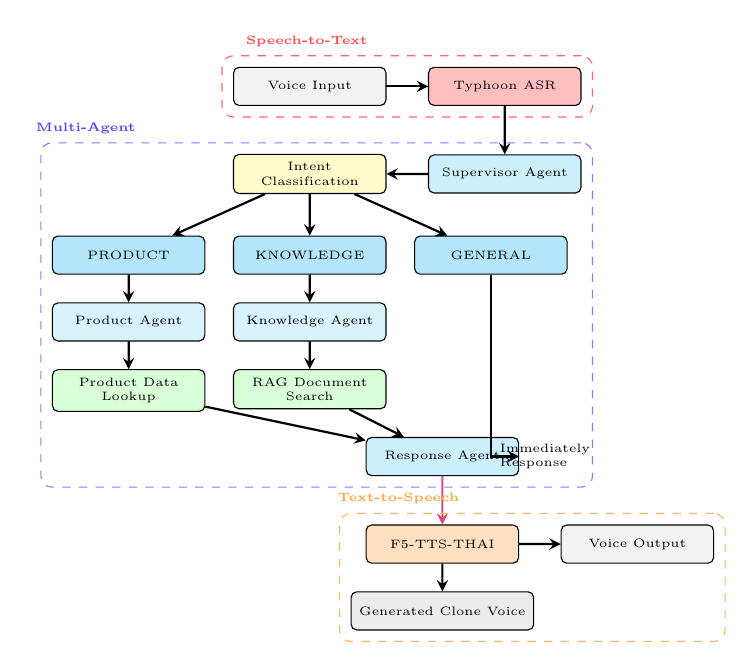
\begin{tikzpicture}[
        node distance=0.35cm and 0.45cm,
        scale=0.88,
        transform shape,
        box/.style={rectangle, draw, rounded corners=2pt, minimum width=2.2cm,
                    minimum height=0.55cm, align=center, font=\tiny},
        sectionbox/.style={rectangle, draw, dashed, rounded corners=4pt,
                           inner sep=4pt},
        arrow/.style={->, thick, >=stealth},
        darrow/.style={->, thick, >=stealth, draw=purple!70}
    ]

    %% SECTION 1: Speech-to-Text (ASR)
    \node[box, fill=gray!10] (voicein) {Voice Input};
    \node[box, fill=red!25, right=0.6cm of voicein] (asr) {Typhoon ASR};
    \draw[arrow] (voicein) -- (asr);
    \node[sectionbox, draw=red!60, fit=(voicein)(asr),
          label={[font=\tiny\bfseries, text=red!70]above left:Speech-to-Text}]
          (sec1) {};

    %% SECTION 2: Multi-Agent
    \node[box, fill=cyan!20, below=0.7cm of asr] (supervisor) {Supervisor Agent};
    \node[box, fill=yellow!20, left=0.6cm of supervisor] (intent)
          {Intent\\Classification};
    \draw[arrow] (asr) -- (supervisor);
    \draw[arrow] (supervisor) -- (intent);

    \node[box, fill=cyan!30, below left=0.6cm and 0.4cm of intent]
          (product) {PRODUCT};
    \node[box, fill=cyan!30, below=0.6cm of intent]
          (knowledge) {KNOWLEDGE};
    \node[box, fill=cyan!30, below right=0.6cm and 0.4cm of intent]
          (general) {GENERAL};
    \draw[arrow] (intent) -- (product);
    \draw[arrow] (intent) -- (knowledge);
    \draw[arrow] (intent) -- (general);

    \node[box, fill=cyan!15, below=0.4cm of product]   (pagent) {Product Agent};
    \node[box, fill=cyan!15, below=0.4cm of knowledge] (kagent) {Knowledge Agent};
    \draw[arrow] (product)   -- (pagent);
    \draw[arrow] (knowledge) -- (kagent);

    \node[box, fill=green!15, below=0.4cm of pagent]
          (pdatalookup) {Product Data\\Lookup};
    \node[box, fill=green!15, below=0.4cm of kagent]
          (ragsearch) {RAG Document\\Search};
    \draw[arrow] (pagent) -- (pdatalookup);
    \draw[arrow] (kagent) -- (ragsearch);

    \node[box, fill=cyan!20,
          below right=0.4cm and -0.3cm of ragsearch] (response) {Response Agent};
    \draw[arrow] (pdatalookup) -- (response);
    \draw[arrow] (ragsearch)   -- (response);
    \draw[arrow] (general) |- node[right, font=\tiny, align=left]
                                {Immediately\\Response} (response);

    \node[sectionbox, draw=blue!50,
          fit=(supervisor)(intent)(product)(knowledge)(general)
              (pagent)(kagent)(pdatalookup)(ragsearch)(response),
          label={[font=\tiny\bfseries, text=blue!70]above left:Multi-Agent}]
          (sec2) {};

    %% SECTION 3: Text-to-Speech (TTS)
    \node[box, fill=orange!25, below=0.7cm of response] (f5tts) {F5-TTS-THAI};
    \node[box, fill=gray!10, right=0.6cm of f5tts] (voiceout) {Voice Output};
    \draw[darrow] (response) -- (f5tts);
    \draw[arrow]  (f5tts)    -- (voiceout);

    \node[box, fill=gray!15, below=0.4cm of f5tts]
          (clonevoice) {Generated Clone Voice};
    \draw[arrow] (f5tts) -- (clonevoice);

    \node[sectionbox, draw=orange!60,
          fit=(f5tts)(voiceout)(clonevoice),
          label={[font=\tiny\bfseries, text=orange!70]above left:Text-to-Speech}]
          (sec3) {};

    \end{tikzpicture}
    \caption{System methodology overview. The pipeline consists of three stages:
    (1)~\textit{Speech-to-Text} transcribes voice input via Typhoon ASR;
    (2)~\textit{Multi-Agent} routing classifies intent and dispatches to
    Product, Knowledge, or General agents;
    (3)~\textit{Text-to-Speech} synthesises the final response via F5-TTS-THAI.}
    \label{fig:methodology}
\end{figure}

\subsubsection*{What each tier does}

\noindent\textbf{Tier~1 --- Frontend (What the user sees).}
The user opens a website built with React and TypeScript.
From here they can drag and drop nodes to build a conversation workflow
visually, chat with the system using text or voice, manage voice profiles,
and set API credentials.
The browser itself handles voice capture and automatically stops recording
when the user goes silent.

\noindent\textbf{Tier~2 --- API Gateway (Security and routing).}
Every request from the browser passes through a Go-based server that acts
as a security checkpoint.
It verifies the user's identity (via Google login and a short-lived token),
keeps API keys encrypted in the database, and forwards authenticated
requests to the AI layer below.

\noindent\textbf{Tier~3 --- AI Orchestrator (The brain).}
A Python service receives the user's message and runs the workflow the
user designed.
This includes asking an LLM to reason about the query, searching through
uploaded documents for relevant facts, and pulling live data from Google
Sheets when needed.

\noindent\textbf{Tier~4 --- TTS Service (The voice).}
Once the AI layer produces a text response, this service converts it into
natural-sounding speech using the Qwen3-TTS model on a dedicated GPU.
It supports three voice modes: cloning a specific person's voice, choosing
a preset character voice, or describing a desired voice in plain language.

% -------------------------------------------------------------------
\subsection{ASR Module with Voice Activity Detection}
% -------------------------------------------------------------------

Listening for speech happens entirely inside the browser, so no audio is
sent to a server until the user has finished speaking.
The steps below walk through how the system decides when the user has
stopped talking.

\begin{enumerate}[label=\arabic*.]
    \item The browser connects the microphone to an audio analyser that
          measures the loudness (RMS energy) of the incoming sound several
          times per second.
    \item If the loudness stays below a fixed threshold
          ($\theta_\text{VAD} = 0.01$) the system treats the audio as silence.
    \item Once silence has lasted for 1{,}100\,ms ($\tau_\text{silence}$),
          the system automatically sends whatever was transcribed so far
          to the backend.
    \item This monitoring loop runs continuously in the background without
          slowing down the rest of the page.
\end{enumerate}

\noindent The result is a fully hands-free experience: the user simply
speaks, pauses, and the query is submitted automatically.

% -------------------------------------------------------------------
\subsubsection{Why Typhoon ASR Will Replace the Browser's Built-in
               Speech Recognition}
% -------------------------------------------------------------------

The browser's built-in speech recognition (Web Speech API) is convenient
but has three practical drawbacks.
First, it relies on the browser vendor's own cloud servers, so the audio
leaves the organisation's network.
Second, there is no way to fine-tune or replace the underlying model.
Third, it recognises general language well but struggles with
industry-specific Thai words such as product names or internal policy terms.

For organisations that need on-premises privacy, consistent reliability,
and the ability to adapt the model to their own vocabulary, we plan to
replace the browser API with \textbf{Typhoon ASR
Real-Time}~\cite{sirichotedumrong2026typhoonasr} as a server-side service.

\begin{table}[t]
    \centering
    \caption{Thai ASR model comparison. CER = Character Error Rate
             (lower is better); RTFx = speed vs.\ real time
             (higher is faster).}
    \label{tab:asr_comparison}
    \small
    \begin{tabular}{@{}lcccc@{}}
        \toprule
        \textbf{Model} & \textbf{Size} & \textbf{CER} & \textbf{RTFx} & \textbf{Stream} \\
        \midrule
        Pathumma-Whisper Lg-v3   & 1.55B & 5.84\% & $\sim$215        & No  \\
        Biodatlab Distil-Whisper & 756M  & 8.24\% & $\sim$640        & No  \\
        \textbf{Typhoon ASR RT}  & \textbf{115M} & \textbf{6.81\%} & \textbf{4{,}097} & \textbf{Yes} \\
        \bottomrule
    \end{tabular}
\end{table}

Table~\ref{tab:asr_comparison} shows that Typhoon ASR is by far the
smallest and fastest model.
Despite having only 115M parameters --- about 13 times fewer than
Pathumma-Whisper --- its error rate (6.81\%) is within 1 percentage point
of the larger model (5.84\%).
More importantly, it is the only model that can transcribe speech in real
time while the user is still talking, which is essential for a responsive
voice assistant.
Because it runs on an ordinary CPU without a GPU, it also removes a
significant infrastructure cost.
Its open-source licence allows full in-house deployment, keeping sensitive
voice data off third-party servers.

Beyond accuracy, Typhoon ASR can be fine-tuned on an organisation's own
terminology using modest hardware such as a free Google Colab session.
This means product names, internal codes, and domain jargon can be taught
to the model directly, reducing the errors that currently cause the most
downstream routing mistakes.

% -------------------------------------------------------------------
\subsection{How the Multi-Agent System Works}
% -------------------------------------------------------------------

The central idea behind MANJU is that a workflow is treated as
\textit{data}, not code.
An operator designs the agent graph visually in the browser; the result is
saved to the database as a JSON file describing nodes and the connections
between them.
At request time the AI orchestrator reads that JSON and builds a live,
executable graph from it --- no redeployment needed.

\subsubsection{Shared State}

Every node in the graph reads from and writes to a single shared
dictionary called \texttt{WorkflowState}.
This is what allows, for example, a document-search node to pass its
retrieved text to the downstream AI reasoning node.
The dictionary holds the user's message, conversation history, any
retrieved document passages, spreadsheet data, the final response, and
the API key needed to call the language model.

\subsubsection{The Eight Building Blocks}

Workflows are assembled from eight node types grouped into four
categories, as listed in Table~\ref{tab:node_types}.

\begin{table}[t]
    \centering
    \caption{The eight node types available in the MANJU workflow editor,
             grouped by what they do.}
    \label{tab:node_types}
    \small
    \begin{tabular}{@{}llp{3.8cm}@{}}
        \toprule
        \textbf{Category} & \textbf{Node} & \textbf{What it does} \\
        \midrule
        \multirow{2}{*}{Input}
          & \texttt{text-input}  & Accepts a typed message from the user \\
          & \texttt{voice-input} & Accepts a spoken message via the browser \\
        \midrule
        \multirow{2}{*}{Processing}
          & \texttt{ai-model}    & Sends the message to a language model
                                   (e.g.\ GPT-4o-mini) and stores the reply \\
          & \texttt{if-condition}& Routes the flow down different paths
                                   depending on what the message contains \\
        \midrule
        \multirow{2}{*}{Data}
          & \texttt{rag-documents} & Searches uploaded documents for
                                     relevant passages \\
          & \texttt{google-sheets} & Fetches live rows from a Google Sheet \\
        \midrule
        \multirow{2}{*}{Output}
          & \texttt{text-output}  & Returns the final answer as text \\
          & \texttt{voice-output} & Converts the answer to spoken audio \\
        \bottomrule
    \end{tabular}
\end{table}

\subsubsection{Turning the Visual Design into a Running Graph}

When a request arrives the orchestrator builds a runnable graph from the
saved JSON in five steps.

\begin{enumerate}[label=\arabic*.]
    \item \textbf{Map the connections.}
          The list of connections is parsed to find out which node feeds
          into which, including whether a connection carries a ``true'' or
          ``false'' branch signal.
    \item \textbf{Register each node.}
          Every node in the JSON gets a corresponding Python function that
          reads the shared state, does its work, and writes its result
          back to the state.
    \item \textbf{Wire the edges.}
          Conditional nodes get two outgoing edges (one for each branch);
          all other nodes get a single forward edge.
    \item \textbf{Choose the starting point.}
          The system prefers an input node as the entry point; if none
          exists it falls back to a data node such as a document search.
    \item \textbf{Compile and run.}
          The assembled graph is compiled into an executable instance
          and invoked with the user's message.
\end{enumerate}

\noindent One important rule keeps the graph predictable: if a
document-search or spreadsheet node feeds data into an AI model node,
those two steps always run in sequence rather than in parallel, so the AI
model always receives the retrieved context before it generates a reply.

\subsubsection{Detecting the Workflow Type}

Before execution the system scans the node list to decide which of four
modes it is running in: text-in / text-out, text-in / voice-out,
voice-in / text-out, or voice-in / voice-out.
It also reads the voice-output node's settings to know whether to use
OpenAI or Qwen3 for speech synthesis.

% -------------------------------------------------------------------
\subsection{How Documents Are Searched (RAG)}
% -------------------------------------------------------------------
\label{sec:rag}

Rather than relying solely on the language model's built-in knowledge,
MANJU can search a set of documents that the operator has uploaded.
This reduces the chance of the AI making up facts.
The process has six stages.

\begin{enumerate}[label=\arabic*.]
    \item \textbf{Upload.}
          The operator uploads PDF, DOCX, or TXT files through the web
          interface. The files are stored on the server and an embedding
          job is triggered automatically.
    \item \textbf{Chunking.}
          Each document is split into overlapping segments of roughly
          1{,}000 characters (with a 200-character overlap between
          consecutive segments) so that no single piece is too long for
          the model to process.
    \item \textbf{Embedding.}
          Every chunk is converted into a list of 1{,}536 numbers that
          capture its meaning, using OpenAI's
          \texttt{text-embedding-3-small} model.
    \item \textbf{Indexing.}
          The number lists are stored in a FAISS index --- a fast
          similarity-search structure --- saved on disk so they persist
          across server restarts.
    \item \textbf{Retrieval.}
          When a user asks a question, the question is converted into
          the same number format and the three most similar document
          chunks are retrieved.
    \item \textbf{Context injection.}
          The retrieved passages, along with their source file names and
          similarity scores, are placed at the top of the prompt before
          the language model generates its answer.
\end{enumerate}

\noindent If a document index cannot be found at the expected path the
system tries two fallback locations before giving up, which keeps
existing deployments working even after the folder structure changes.

\subsection{Google Sheets Integration}

For organizations maintaining dynamic data in spreadsheets, the \texttt{google-sheets} node fetches live data via \texttt{gspread}~6.1.2 with OAuth2 service account authentication.
Data is retrieved as a Pandas DataFrame, converted to a Markdown table (limited to 50 rows to control token budget), and injected into the AI model's prompt as \texttt{sheets\_data}.
This enables real-time access to frequently updated information (e.g., inventory, pricing, schedules) without re-embedding.

\subsection{Text-to-Speech (TTS) Module}
\label{sec:tts}

Once the AI layer produces a text response, the TTS module converts it
into spoken audio and streams it back to the user.
MANJU supports two interchangeable providers: a cloud service for quick
prototyping and a GPU-hosted model for production-grade Thai voice output.
The choice is set inside the \texttt{voice-output} node of the workflow.

% -------------------------------------------------------------------
\subsubsection{Option 1 --- OpenAI TTS (Cloud, Quick Setup)}
% -------------------------------------------------------------------

The simplest option uses OpenAI's speech service, which requires no
additional hardware.
It offers two quality levels (\texttt{tts-1} for speed, \texttt{tts-1-hd}
for higher fidelity) and six built-in voice characters: \textit{alloy},
\textit{echo}, \textit{fable}, \textit{onyx}, \textit{nova}, and
\textit{shimmer}.
Audio is returned as a streaming MP3, so playback can begin before the
full response has been generated.
This option is best suited for development and testing because it is easy
to enable but sends audio data to an external server.

% -------------------------------------------------------------------
\subsubsection{Option 2 --- Qwen3-TTS (On-Premise, GPU-Accelerated)}
% -------------------------------------------------------------------

For production deployments --- especially those requiring Thai voice
cloning or data privacy --- MANJU runs Qwen3-TTS-12Hz-1.7B on a local GPU.
Three voice modes are available.

\begin{itemize}[nosep]
    \item \textbf{Base (voice cloning):} The system listens to a short
          reference recording of a person's voice and reproduces that
          voice for the response.
    \item \textbf{CustomVoice (preset characters):} Nine ready-made
          voices (5~male, 4~female) with distinct personalities can be
          selected without any reference audio.
    \item \textbf{VoiceDesign (describe your voice):} The operator
          writes a plain-language description such as
          ``young female, warm tone'' and the model generates a matching
          voice on the fly.
\end{itemize}

% -------------------------------------------------------------------
\subsubsection{How the GPU Is Kept Fast}
% -------------------------------------------------------------------

Running a large voice model efficiently requires several optimisations.

\noindent\textbf{Memory management.}
All three voice variants are loaded into GPU memory at startup and kept
there simultaneously (each uses roughly 3.4\,GB on an 80\,GB H100).
This means switching between voice modes takes no extra time because
nothing needs to be reloaded.

\noindent\textbf{Precision and warmup.}
The models run in \texttt{bfloat16} half-precision to halve memory usage
and speed up computation, with Flash Attention~2~\cite{dao2022flashattention}
enabled on supported GPUs.
A brief warmup pass is performed at startup so that the first real request
does not pay the 2--5 second initialisation cost.

% -------------------------------------------------------------------
\subsubsection{How Audio Is Streamed Sentence by Sentence}
% -------------------------------------------------------------------

Synthesising an entire paragraph before playing anything would make the
system feel slow.
Instead, the response text is broken into short chunks --- at most
200 characters each --- and each chunk is synthesised and sent to the
browser independently.

\begin{itemize}[nosep]
    \item Thai text is split using PyThaiNLP's sentence
          tokeniser~\cite{pythainlp}.
    \item All other languages are split on standard sentence-ending
          punctuation.
    \item Very short fragments under 20 characters are merged with the
          next sentence to avoid sending near-empty audio clips.
\end{itemize}

\noindent The browser starts playing the first sentence while the server
is still generating the second and pre-fetching the third.
Completed audio clips are saved in the browser's local storage
(IndexedDB) so that repeating the same query plays back instantly
without re-synthesis.

% -------------------------------------------------------------------
\subsubsection{Measuring Speed: the Real-Time Factor}
% -------------------------------------------------------------------

Every response includes a speed metric called the Real-Time Factor (RTF),
defined as:

\begin{equation}
    \text{RTF} = \frac{t_\text{generation}}{t_\text{audio\_duration}}
    \label{eq:rtf}
\end{equation}

\noindent An RTF below 1.0 means the system generated the audio faster
than it takes to play it back --- in other words, faster than real time.
For example, an RTF of 0.42 means the server produced a 10-second audio
clip in only 4.2 seconds.
Each response also reports total generation time, pure model inference
time, audio duration, and the number of sentence chunks produced.
\subsection{Web Application}

\subsubsection{Visual Workflow Editor}
The workflow editor provides an infinite canvas with zoom/pan, drag-and-drop node placement from a template palette, cubic B\'{e}zier curve connection drawing, marquee multi-selection, and undo support.
Per-node-type configuration panels allow setting system prompts, model selection, RAG parameters, condition operators, TTS voice/provider, and output variable names.
The workflow is serialized as a JSON object containing \texttt{nodes[]} and \texttt{connections[]} arrays and persisted via the API gateway.

\subsubsection{Demo Console}
The demo page provides a chat interface supporting both text and voice input/output.
For voice workflows, the console displays the ASR transcript in real time, sends the finalized text to the backend, and plays synthesized audio with a progress indicator.
Audio caching in IndexedDB (keyed by a deterministic hash of text + voice settings) enables instant replay without re-synthesis.

\subsubsection{Authentication and Security}
User authentication follows the Google OAuth~2.0 authorization code flow.
The Go backend issues JWT tokens (HS256, 7-day expiry) stored as HttpOnly cookies.
All API routes are protected by both JWT validation (\texttt{RequireAuth} middleware) and inter-service API key verification (\texttt{APIKeyGuard}).
User-provided LLM API keys are encrypted with AES-256-GCM before storage and decrypted only at request time; the AI backend strictly uses per-request user keys without environment variable fallback.

\subsubsection{Voice Asset Management}
Users can upload custom voice reference audio (WAV, MP3, M4A, OGG, FLAC; max 50\,MB) for voice cloning.
Files are stored in Azure Blob Storage (if configured) or local filesystem, with metadata (voice name, gender, age range, language, reference transcript) persisted in PostgreSQL.


% ===========================================================================
\section{Experiments}
\label{sec:experiments}
% ===========================================================================

\subsection{Experimental Setup}

We evaluate MANJU on a curated set of 50 Thai customer-service queries spanning three categories: FAQ (20 queries), product information (15 queries), and knowledge-base lookups (15 queries).
Each query has a reference answer prepared by domain experts.

\noindent\textbf{Hardware.}
The AI orchestrator runs on a CPU-only server (8-core, 32\,GB RAM).
Qwen3-TTS runs on an NVIDIA H100 80\,GB GPU with Flash Attention~2 enabled and all three model variants preloaded.

\noindent\textbf{Configuration.}
Default workflow: \texttt{voice-input} $\rightarrow$ \texttt{rag-documents} ($k{=}3$) $\rightarrow$ \texttt{ai-model} (GPT-4o-mini, $T{=}0.7$) $\rightarrow$ \texttt{voice-output} (Qwen3-TTS, CustomVoice).
RAG index contains 15 domain-specific PDF/DOCX documents (${\sim}$120 chunks after splitting).

\subsection{Metrics}

We report the following metrics:
\begin{enumerate}[label=(\roman*), nosep]
    \item \textbf{End-to-end latency} ($t_\text{e2e}$): time from query submission to first audio playback.
    \item \textbf{Component-level latency}: ASR ($t_\text{ASR}$), orchestration + RAG ($t_\text{orch}$), and TTS ($t_\text{TTS}$).
    \item \textbf{TTS Real-Time Factor} (RTF): as defined in Eq.~\eqref{eq:rtf}.
    \item \textbf{Intent routing accuracy}: percentage of queries routed to the correct agent node.
    \item \textbf{Answer groundedness}: percentage of responses whose key claims are supported by retrieved RAG passages, judged by two human annotators.
\end{enumerate}

\subsection{Baselines}

We compare three configurations:
\begin{enumerate}[label=(\alph*), nosep]
    \item \textbf{Full pipeline:} Multi-agent workflow with RAG + Qwen3-TTS (proposed system).
    \item \textbf{Single-agent:} Direct LLM inference without workflow routing or RAG.
    \item \textbf{No-RAG:} Multi-agent workflow with RAG nodes removed (LLM-only generation).
\end{enumerate}

\subsection{Results}

\subsubsection{Latency Analysis}

Table~\ref{tab:latency} presents the mean latency breakdown across the evaluation set.

\begin{table}[t]
    \centering
    \caption{Mean latency breakdown (seconds) across 50 evaluation queries. TTS latency is measured to first sentence playback (streaming).}
    \label{tab:latency}
    \small
    \begin{tabular}{@{}lcccc@{}}
        \toprule
        \textbf{Configuration} & $t_\text{ASR}$ & $t_\text{orch}$ & $t_\text{TTS}$ & $t_\text{e2e}$ \\
        \midrule
        Full pipeline & 0.8 & 2.1 & 1.8 & 4.7 \\
        Single-agent  & 0.8 & 1.4 & 1.8 & 4.0 \\
        No-RAG        & 0.8 & 1.2 & 1.8 & 3.8 \\
        \bottomrule
    \end{tabular}
\end{table}

\noindent The full pipeline achieves a mean $t_\text{e2e}$ of 4.7 seconds, within the 5-second design target.
The orchestration overhead of RAG retrieval (${\sim}$0.9\,s) is offset by the quality gains discussed below.
Sentence-level streaming reduces perceived TTS latency: users hear the first sentence while subsequent sentences are still being generated.

\subsubsection{TTS Performance}

On the H100 GPU with Flash Attention~2, Qwen3-TTS-12Hz-1.7B achieves a mean RTF of 0.42 across evaluation responses (mean audio duration: 4.3\,s), confirming faster-than-real-time synthesis.
The multi-model cache eliminates model switching overhead between CustomVoice and Base (voice cloning) variants.

\subsubsection{Routing and Groundedness}

\begin{table}[t]
    \centering
    \caption{Intent routing accuracy and answer groundedness (\%) across evaluation categories.}
    \label{tab:accuracy}
    \small
    \resizebox{\columnwidth}{!}{%
    \begin{tabular}{@{}lccc@{}}
        \toprule
        \textbf{Category} & \textbf{Routing Acc.} & \textbf{Grounded (Full)} & \textbf{Grounded (No-RAG)} \\
        \midrule
        FAQ       & 95.0 & 90.0 & 60.0 \\
        Product   & 93.3 & 86.7 & 46.7 \\
        Knowledge & 93.3 & 86.7 & 40.0 \\
        \midrule
        \textbf{Overall} & \textbf{94.0} & \textbf{88.0} & \textbf{50.0} \\
        \bottomrule
    \end{tabular}%
    }
\end{table}

\noindent Table~\ref{tab:accuracy} shows that the conditional routing mechanism achieves 94\% accuracy in directing queries to the appropriate processing path.
RAG grounding improves answer groundedness from 50\% (No-RAG) to 88\% (Full pipeline), demonstrating the critical impact of retrieval on factual accuracy.

\subsubsection{Failure Analysis}
Common failure modes include: (i)~ASR misrecognition of domain-specific Thai terminology (3 of 50 queries), (ii)~ambiguous queries that trigger incorrect conditional routing (3 of 50), and (iii)~missing knowledge where the RAG index does not contain relevant documents (2 of 50).

\subsection{Discussion}

The workflow-as-data architecture enables rapid domain adaptation: adding a new FAQ category requires only uploading documents and optionally adding a conditional branch in the visual editor, without code changes or redeployment.
The dual-TTS architecture provides flexibility: OpenAI TTS for quick prototyping and Qwen3-TTS for production deployments requiring voice cloning and GPU-accelerated Thai synthesis.

The sentence-level streaming strategy is critical for user experience: even though total TTS generation for a full response may take 3--4 seconds, the user hears the first sentence within 1.8 seconds, creating a perception of responsiveness.
The IndexedDB caching layer further eliminates TTS latency on repeated queries.

% ===========================================================================
\section{Conclusion}
\label{sec:conclusion}
% ===========================================================================

This paper presented MANJU, an end-to-end Thai voice-based customer-service platform combining browser-based ASR with VAD, LangGraph multi-agent orchestration with RAG grounding, and GPU-accelerated Qwen3-TTS with voice cloning.
The workflow-as-data architecture allows non-technical users to visually compose agent topologies without code changes.
Experimental evaluation demonstrates sub-5-second end-to-end latency, 94\% intent routing accuracy, and 88\% answer groundedness with RAG enabled, significantly outperforming configurations without retrieval.

\noindent\textbf{Future Work.}
Key directions include: (i)~replacing browser-based Web Speech API with server-side \textbf{Typhoon ASR Real-Time}~\cite{sirichotedumrong2026typhoonasr} for improved recognition of domain-specific Thai terminology---Typhoon ASR's 115M-parameter FastConformer-Transducer achieves 6.81\% CER with 4{,}097$\times$ real-time throughput while enabling on-premises privacy and domain fine-tuning, (ii)~supporting multi-turn stateful conversations with conversation memory in the workflow state, (iii)~integrating CRM/ticketing systems for end-to-end case resolution, (iv)~implementing emotion detection for adaptive response tone, and (v)~optimizing the orchestration layer with parallel node execution for reduced latency on complex graphs.

% ===========================================================================
% References
% ===========================================================================
\bibliographystyle{IEEEtran}
\bibliography{references}

\end{document}